

\documentclass[a5paper]{article}

% Requires PGF >=  1.09
% Note:
%   This example works only with pdftex >= 1.30.0
%   You have to run pdftex on the example twice!
\usepackage{amsmath}
\usepackage{tikz}

\begin{document}
\thispagestyle{empty}

Lorem ipsum dolor sit amet, consectetuer adipiscing elit. Donec luctus 
mollis nisl. Nullam tempor, diam non tincidunt tincidunt, nunc tortor 
elementum odio, nec iaculis urna leo a eros. Lorem ipsum dolor sit amet,
consectetuer adipiscing elit. Sed elit elit, pellentesque et, 
sollicitudin a, imperdiet eget, tellus. Vestibulum et sapien. Maecenas 
libero. Vivamus vel metus in ipsum ultricies commodo. Donec quam. Fusce 
arcu. In est felis, sagittis vitae, vehicula ut, tristique vitae, eros. 
Mauris ut lorem vel risus posuere elementum. Quisque volutpat ornare lorem. 
Integer porta.
\begin{multline}\label{eq:steeringfull}
    \begin{bmatrix}
        m-Y_{\dot{v}} & Y_{\dot{r}} & 0\\
        -N_{\dot{v}} & I_z-N_{\dot{r}} & 0\\
        0 & 0 & 1
    \end{bmatrix}
    \begin{bmatrix}
        \dot{v} \\ \dot{r}\\ \dot{\psi}
    \end{bmatrix}\\ +
    \begin{bmatrix}
        -Y_v & -Y_r+mu_0\\
        -N_v & -N_r & 0\\
        0 & -1 & 0
    \end{bmatrix}
    \begin{bmatrix}
        v \\ r \\ \psi
    \end{bmatrix} =
    \begin{bmatrix}
        Y_\delta \\ N_\delta \\ 0
    \end{bmatrix}\delta_r
\end{multline}

Donec ut neque vel leo sagittis tristique. Cras et justo. Mauris lorem 
purus, sagittis eu, consectetuer et, lacinia et, augue. Ut in velit in 
diam semper rutrum. Nunc rhoncus. Cras tincidunt. Aenean nec quam. In commodo
sem ac nulla. Donec fermentum metus non nisl sagittis sagittis. Vestibulum 
sit amet nunc. Vivamus dapibus congue purus. Quisque arcu tellus, 
pellentesque ac, tincidunt lobortis, commodo ac, purus.


% Start of the interesting part
% If you place the code at the beginning of the page, the image will be
% put behind the text.
%
% The overlay option removes the picture from the ordinary page flow. 
\begin{tikzpicture}[remember picture, overlay]
    \node[inner sep=0pt] at (current page.center) {%
        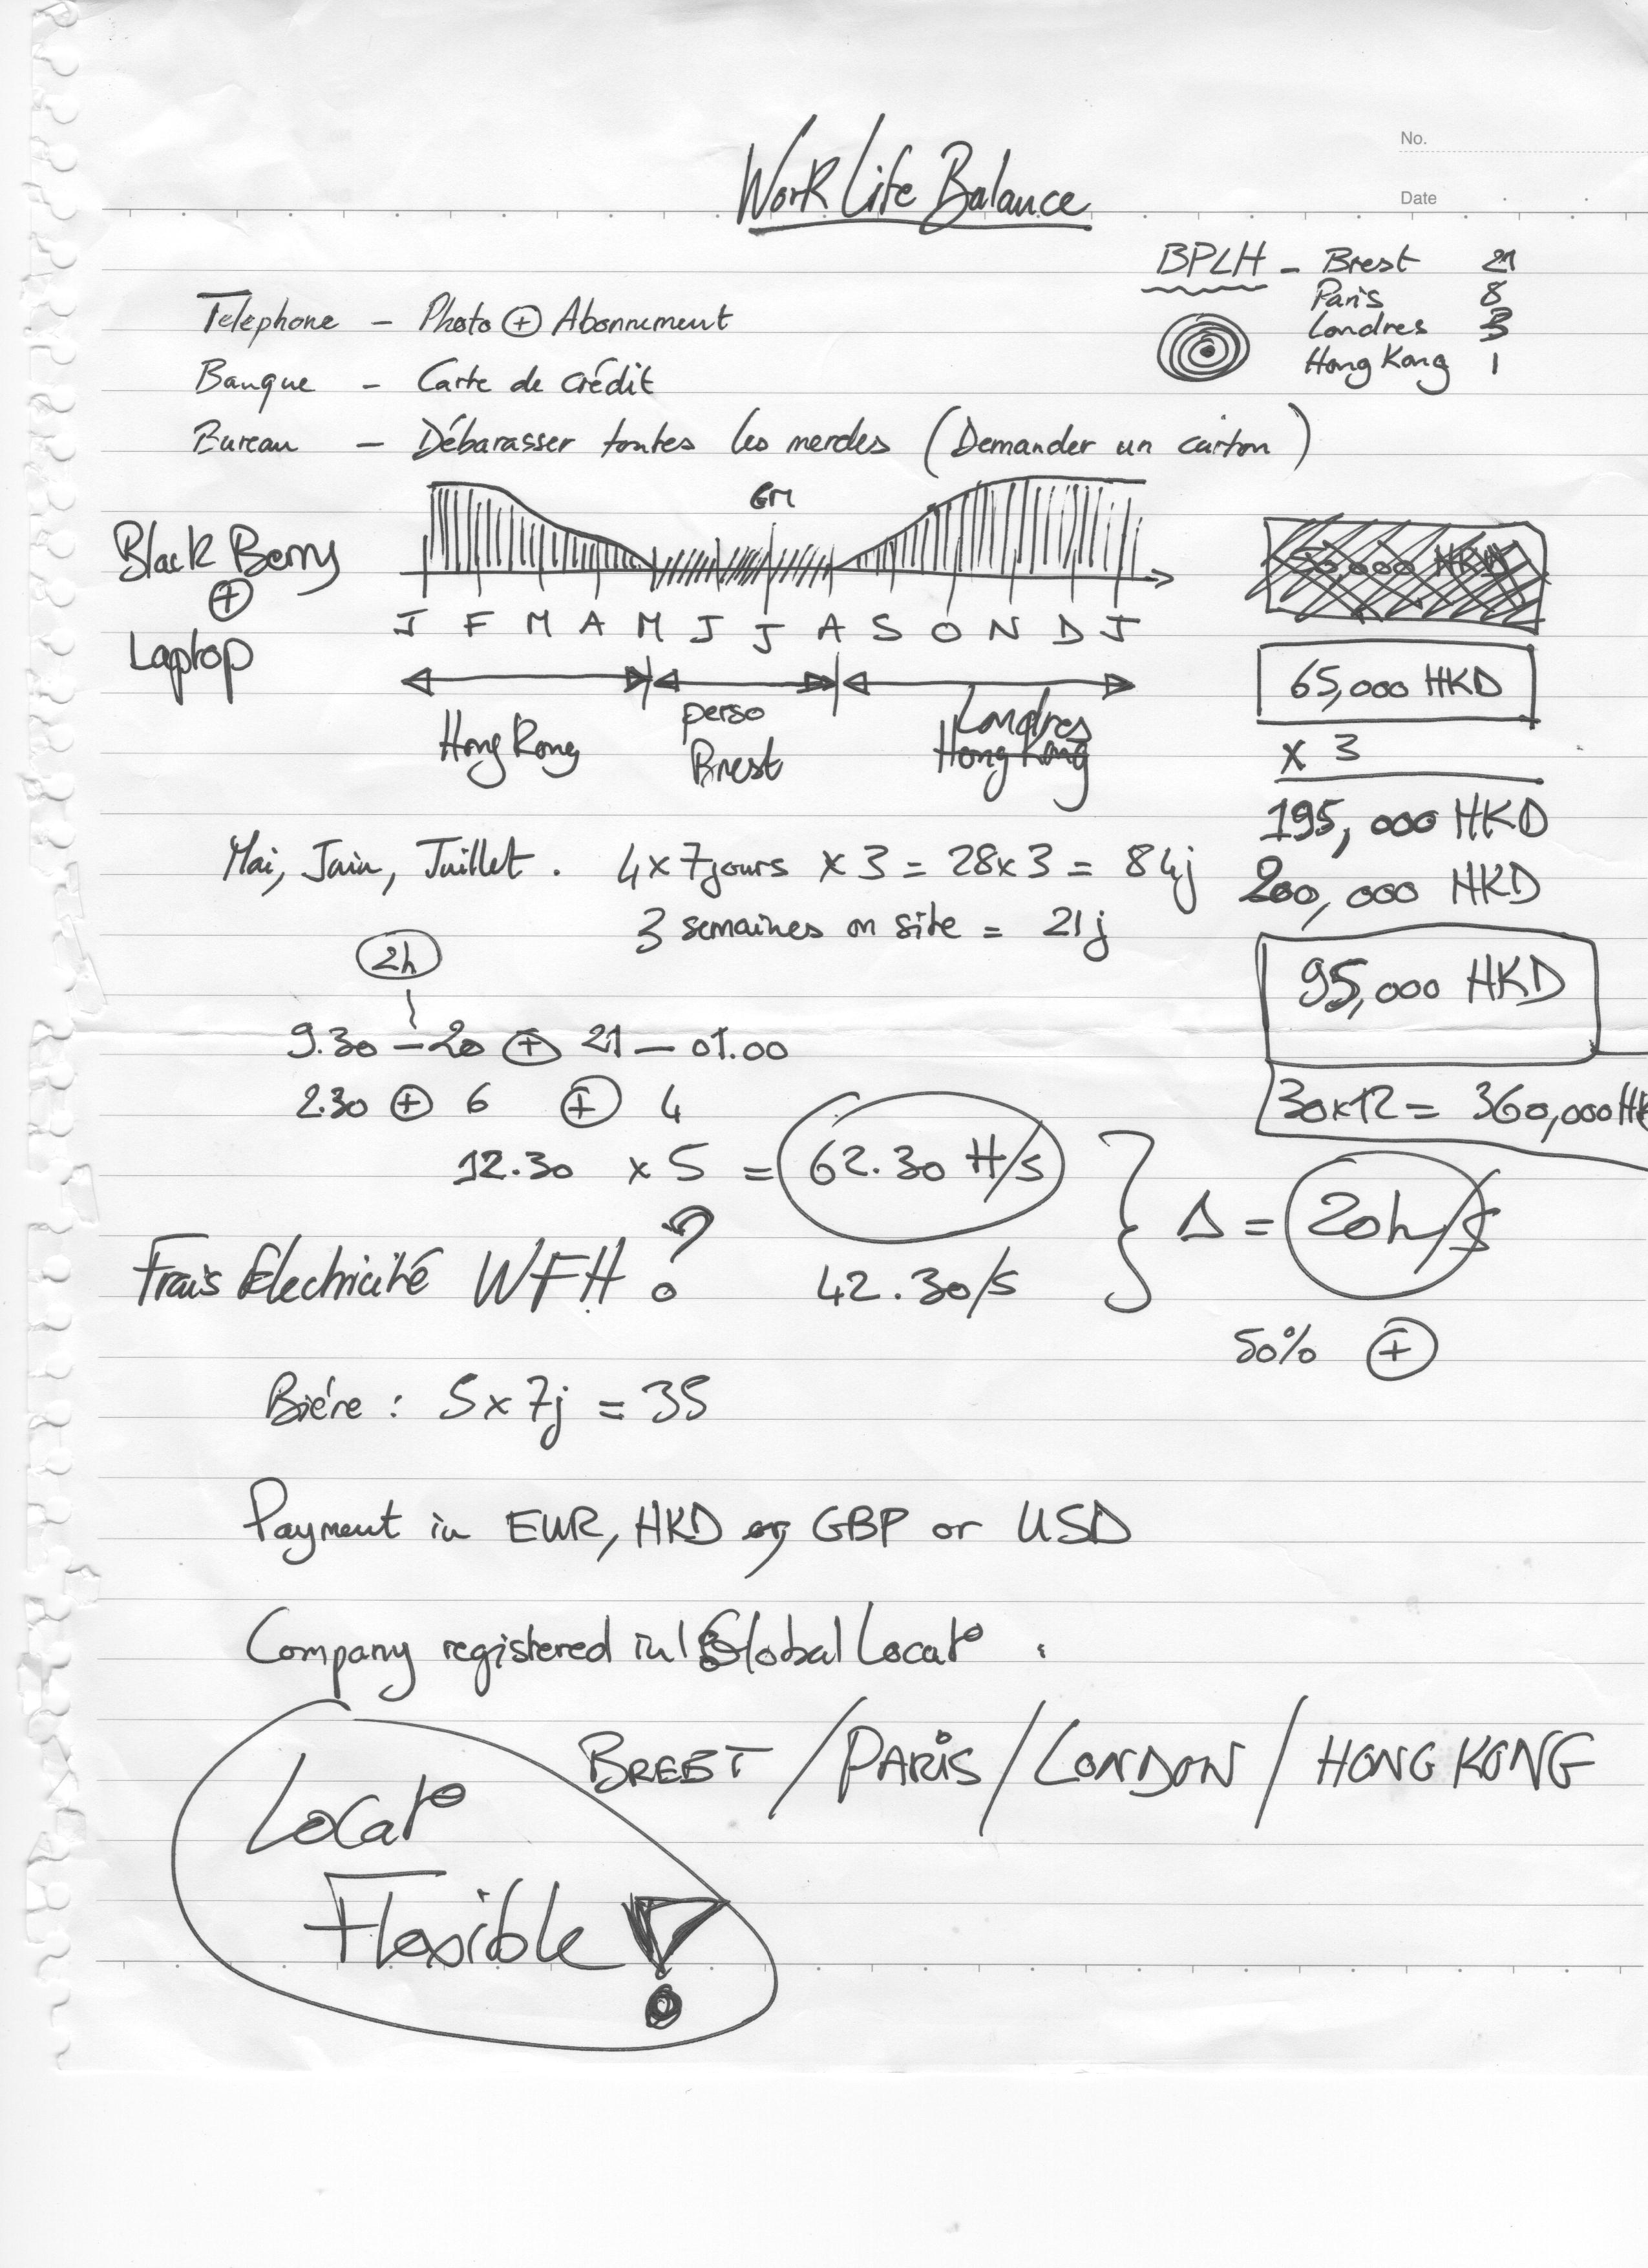
\includegraphics[width=\paperwidth,height=\paperheight]{007}%
    };%
\end{tikzpicture}


\end{document}

